\chapter{Métabolismes microbiens et biofilms}\label{ch:b2:microbial-metabolism}

Remplissez une éprouvette de verre de vase de mare, d'un peu de papier
déchiqueté, d'un jaune d'œuf et d'eau, et laissez-la sur un rebord de
fenêtre. En quelques semaines, elle se stratifie en bandes colorées~:
des algues vertes en haut, une couche couleur rouille, une bande
pourpre, une bande verte plus bas, et une vase noire de sulfure au fond.
Rien n'a été ajouté, sinon de la lumière. Chaque bande est une
population qui vit d'une chimie différente --- du dioxygène, du nitrate,
du sulfate, du sulfure, du dihydrogène --- et chacune nourrit la
suivante. La colonne est le monde microbien en miniature~: des cellules
qui tirent leur énergie de presque n'importe quel couple de substances
capables d'échanger des électrons et qui, ensemble, font tourner les
cycles chimiques de la planète. Ce chapitre expose la logique de cette
énergétique, la cinétique de la croissance microbienne, et la vie
collective des microbes sur les surfaces, qui est la façon dont la
plupart d'entre eux vivent réellement.

\section{Les manières de gagner sa vie}

\begin{definition}[Types trophiques]\label{def:b2:microbial-metabolism:trophic}
\index{chimiotrophe}\index{phototrophe}\index{lithotrophe}\index{organotrophe}
Un organisme se classe d'après trois réponses. Sa \emph{source
d'énergie}~: la lumière (\emph{phototrophe}) ou des réactions chimiques
(\emph{chimiotrophe}). Sa \emph{source d'électrons}~: des substances
minérales --- $\mathrm{H_2}$,
$\mathrm{H_2S}$, $\mathrm{NH_4^+}$, $\mathrm{Fe^{2+}}$, l'eau ---
(\emph{lithotrophe}) ou des molécules organiques (\emph{organotrophe}).
Sa \emph{source de carbone}~: le $\mathrm{CO_2}$ (\emph{autotrophe}) ou
du carbone organique (\emph{hétérotrophe}). Les plantes et les
cyanobactéries sont photolithoautotrophes~; les animaux, les champignons
et \emph{E.~coli} sont chimioorganohétérotrophes~; les bactéries
nitrifiantes et sulfo-oxydantes sont chimiolithoautotrophes~: elles
fabriquent leur matière organique à partir du
$\mathrm{CO_2}$ avec une énergie tirée de l'oxydation de minéraux, à
l'obscurité. Presque toutes les combinaisons existent quelque part chez
les \omterm{def:b2:unicellular-diversity:prokaryote}{procaryotes}~; les eucaryotes n'en occupent que deux.
\end{definition}

\begin{theorem}[L'énergie d'un couple redox]\label{thm:b2:microbial-metabolism:redox}
\index{potentiel redox}\index{tour a electrons@tour à électrons}
Tout métabolisme producteur d'énergie fait passer des électrons d'un
couple \emph{donneur} à un couple \emph{accepteur}. Chaque couple a un
potentiel standard $E^{\circ\prime}$ (à pH 7)~: plus il est négatif,
plus le couple cède facilement ses électrons. Le transfert de $n$ moles
d'électrons d'un donneur de potentiel $E_d$ à un accepteur de potentiel
$E_a$ libère une énergie libre standard
\[
\Delta G^{\circ\prime} = -\,n F\,(E_a - E_d), \qquad F = \qty{96.5}{kJ/V/mol},
\]
de sorte que le rendement est proportionnel à la distance verticale
entre les deux couples sur la \emph{\omterm{thm:b2:microbial-metabolism:redox}{tour à électrons}}. Avec
$\mathrm{O_2/H_2O}$ à \qty{+0.82}{V} et $\mathrm{CO_2}$/glucose à
\qty{-0.43}{V}, les 24 électrons d'une molécule de glucose fournissent
$24\times 96.5\times 1.25 = \qty{2900}{kJ/mol}$~; cédés plutôt au
sulfate ($\mathrm{SO_4^{2-}/H_2S}$, \qty{-0.22}{V}), les mêmes
électrons ne fournissent que $24\times 96.5\times 0.21 = \qty{490}{kJ/mol}$.
\end{theorem}
\begin{proof}
Pour la réaction donneur$_{\text{réd}}$ + accepteur$_{\text{ox}}$
$\to$ donneur$_{\text{ox}}$ + accepteur$_{\text{réd}}$, la variation
d'énergie libre est le travail fourni par $n$ moles de charge
électronique $nF$ qui descendent la différence de potentiel
$E_a - E_d$, avec la convention de signe selon laquelle un transfert
spontané (des électrons vers le couple le plus positif) a
$\Delta G < 0$. C'est la relation de Nernst du volume de première année
appliquée à deux demi-réactions.
\end{proof}

\begin{omfigure}
\begin{tikzpicture}[every node/.style={font=\scriptsize}, y=6cm]
  \draw[thick, ->] (0,-0.55) -- (0,0.95) node[above] {$E^{\circ\prime}$ (V)};
  \foreach \v in {-0.4,-0.2,0,0.2,0.4,0.6,0.8} \draw (-0.08,\v) -- (0.08,\v) node[right, xshift=0.05cm] {\v};
  % donors on the right: value/label position/text
  \foreach \v/\y/\l in {-0.43/-0.49/{$\mathrm{CO_2}$/glucose}, -0.42/-0.40/{$2\mathrm{H^+/H_2}$}, -0.32/-0.31/{$\mathrm{NAD^+/NADH}$}, -0.27/-0.22/{$\mathrm{S^0/H_2S}$}, 0.03/0.03/{fumarate/succinate}, 0.34/0.34/{$\mathrm{NO_2^-/NH_4^+}$}}
    { \draw[omDef, thick] (0.8,\v) -- (1.6,\v); \draw[omDef] (1.6,\v) -- (1.85,\y); \node[omDef, anchor=west] at (1.9,\y) {\l}; }
  % acceptors on the left
  \foreach \v/\y/\l in {-0.24/-0.29/{$\mathrm{CO_2/CH_4}$}, -0.22/-0.17/{$\mathrm{SO_4^{2-}/H_2S}$}, 0.43/0.43/{$\mathrm{NO_3^-/NO_2^-}$}, 0.74/0.69/{$\mathrm{NO_3^-/N_2}$}, 0.77/0.77/{$\mathrm{Fe^{3+}/Fe^{2+}}$}, 0.82/0.86/{$\mathrm{O_2/H_2O}$}}
    { \draw[omThm, thick] (-1.6,\v) -- (-0.8,\v); \draw[omThm] (-1.6,\v) -- (-1.85,\y); \node[omThm, anchor=east] at (-1.9,\y) {\l}; }
  \node[omThm, anchor=south] at (-2.4,0.93) {accepteurs};
  \node[omDef, anchor=south] at (2.4,0.93) {donneurs};
  % arrows showing two metabolisms
  \draw[->, very thick, omExo!80!black] (4.9,-0.43) -- (4.9,0.80);
  \node[anchor=west, align=left] at (5.0,0.2) {respiration aérobie\\du glucose~: \qty{1.25}{V},\\\qty{2900}{kJ/mol}};
  \draw[->, very thick, omProp] (4.2,-0.43) -- (4.2,-0.24);
  \node[anchor=north, align=center] at (4.2,-0.52) {sulfato-réduction~:\\\qty{0.21}{V}, \qty{490}{kJ/mol}};
  \draw[dashed, gray] (3.5,-0.43) -- (4.9,-0.43);
  \draw[dashed, gray] (3.5,0.82) -- (4.9,0.82);
  \draw[dashed, gray] (3.5,-0.22) -- (4.2,-0.22);
\end{tikzpicture}

{\small La \omterm{thm:b2:microbial-metabolism:redox}{tour à électrons}. Les donneurs (en bleu) sont placés à leur
potentiel standard~; les accepteurs (en rouge) de même. Un métabolisme
est une chute d'un donneur vers un accepteur situé au-dessus de lui, et
son rendement énergétique est proportionnel à la hauteur de la chute~:
du glucose au dioxygène, la chute est longue~; du glucose au sulfate,
elle est courte.}
\end{omfigure}

\begin{proposition}[La chimiolithotrophie]\label{prop:b2:microbial-metabolism:lithotrophy}
\index{chimiolithotrophie}\index{nitrification}
Certaines bactéries tirent toute leur énergie d'oxydations minérales,
avec le dioxygène (ou le nitrate) comme accepteur, et fixent le
$\mathrm{CO_2}$ grâce à l'ATP et au pouvoir réducteur ainsi obtenus.
Les \emph{nitrifiants}~: les oxydants de l'ammonium
(\emph{Nitrosomonas}) transforment $\mathrm{NH_4^+}$ en nitrite
($\Delta G^{\circ\prime} = \qty{-275}{kJ/mol}$), les oxydants du nitrite
(\emph{Nitrobacter}) transforment le nitrite en nitrate
(\qty{-74}{kJ/mol})~; ensemble, ils convertissent l'ammonium de la
décomposition en nitrate absorbé par les plantes
(\cref{ch:b2:biogeochemical-cycles}).
Les \emph{sulfo-oxydants} (\emph{Thiobacillus}, \emph{Beggiatoa})
oxydent $\mathrm{H_2S}$ en soufre et en sulfate~; les
\emph{ferro-oxydants} oxydent $\mathrm{Fe^{2+}}$ en rouille~; les
\emph{hydrogéno-oxydants} brûlent le
$\mathrm{H_2}$. Comme leurs donneurs d'électrons sont situés haut sur
la tour, le rendement par molécule est faible, et comme ces donneurs
sont des réducteurs plus faibles que le NADH, ces bactéries doivent
dépenser de l'énergie pour faire \emph{remonter} les électrons afin de
produire le NADH dont la fixation du carbone a besoin~: un nitrifiant
oxyde une trentaine d'ions ammonium pour fixer un
$\mathrm{CO_2}$, et croît lentement.
\end{proposition}
\begin{proof}[Faits expérimentaux]
Winogradsky (1887--1890) cultiva des bactéries sulfureuses
filamenteuses dans une goutte d'eau où il laissait diffuser du sulfure
d'un côté et de l'air de l'autre~: elles se rassemblaient à la
frontière, accumulaient des granules de soufre et les consommaient
lorsqu'on coupait l'arrivée de sulfure. Il isola ensuite des bactéries
nitrifiantes sur un milieu purement minéral contenant de l'ammonium et
aucun carbone organique, sur lequel elles croissaient en produisant du
nitrate --- première démonstration que la vie peut se construire à
partir du $\mathrm{CO_2}$ et de l'énergie d'une réaction minérale,
sans lumière. Il nomma ce processus chimiosynthèse.
\end{proof}

\begin{omfigure}
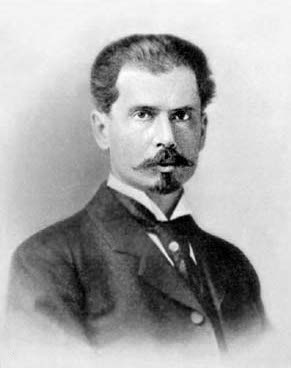
\includegraphics[width=0.26\linewidth]{images/book4/winogradsky.jpg}\hspace{0.05\linewidth}
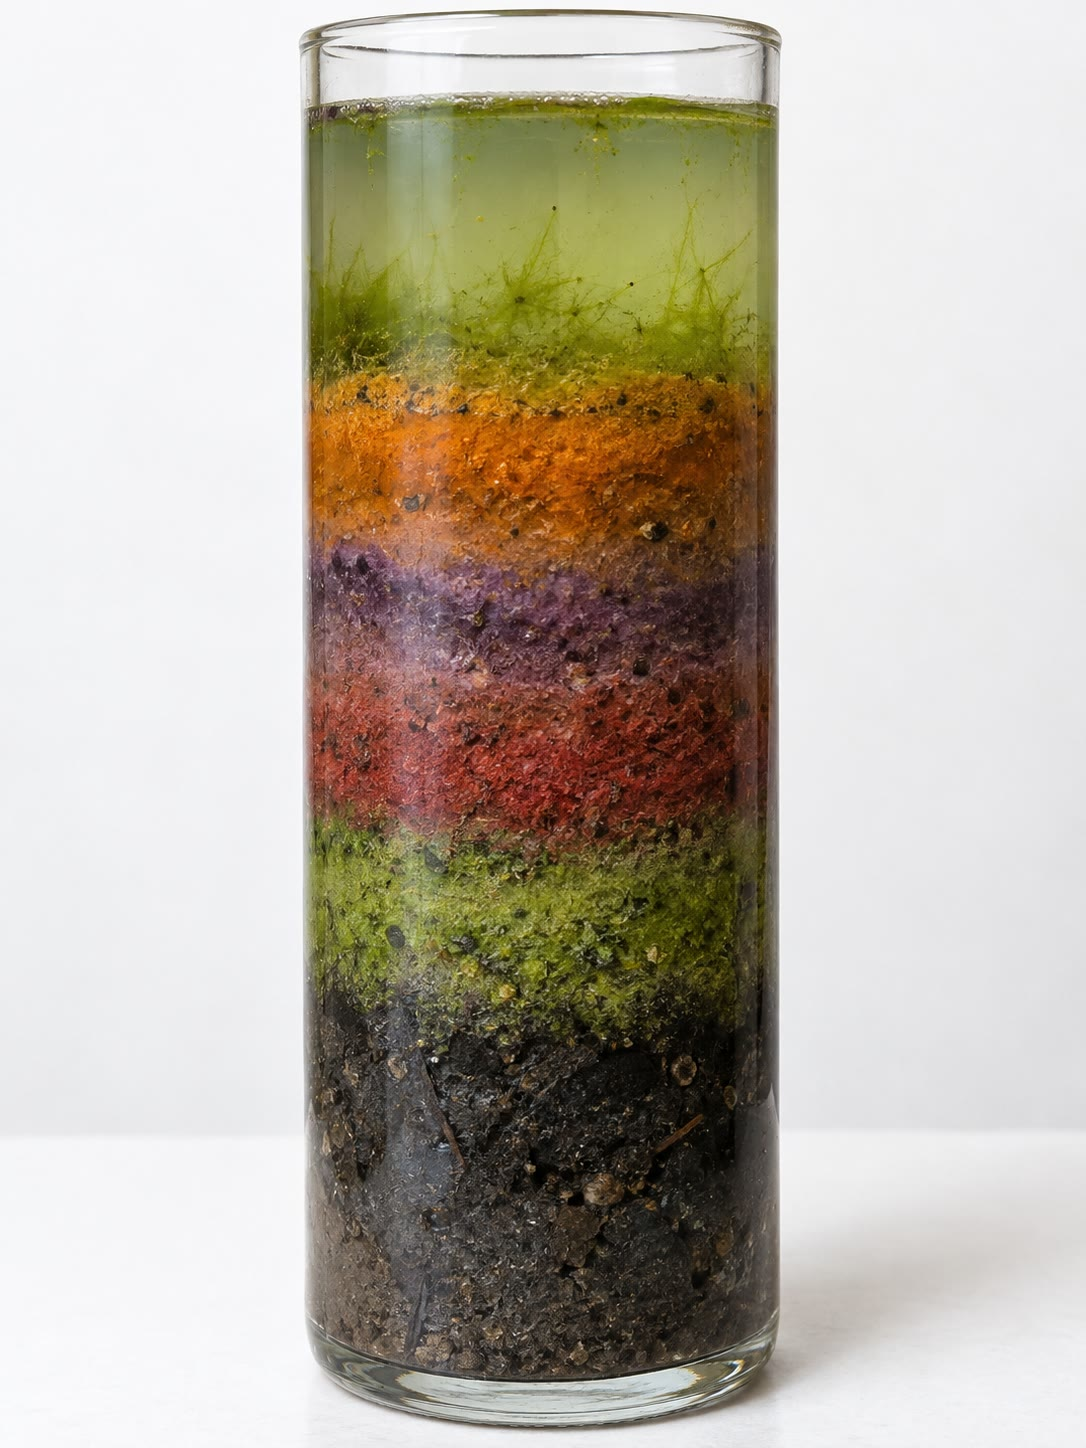
\includegraphics[width=0.30\linewidth]{images/book4/ai/b4-02-winogradsky-column.jpg}

{\small Sergueï Winogradsky, qui découvrit la \omterm{def:b2:microbial-metabolism:trophic}{chimiolithotrophie}, et la
colonne qui porte son nom~: un cylindre de vase et d'eau qui se
stratifie à la lumière en bandes d'algues, de ferro-oxydants et de
sulfo-oxydants, de bactéries pourpres et vertes sulfureuses, et de
sulfato-réducteurs dans la vase noire.}
\end{omfigure}

\begin{definition}[La photosynthèse anoxygénique]\label{def:b2:microbial-metabolism:anoxygenic}
\index{photosynthese anoxygenique@photosynthèse anoxygénique}
Les bactéries pourpres et vertes font la photosynthèse avec un seul
photosystème et une bactériochlorophylle qui absorbe dans le proche
infrarouge, en utilisant $\mathrm{H_2S}$, $\mathrm{H_2}$ ou des acides
organiques comme donneurs d'électrons au lieu de l'eau~: elles libèrent
du soufre ou du sulfate, jamais de dioxygène, et elles ont besoin d'une
lumière de longueurs d'onde qui traversent la couche d'algues vertes et
de cyanobactéries située au-dessus d'elles. Les bactéries pourpres
sulfureuses croissent donc dans la bande pourpre de la colonne de
Winogradsky, exactement là où le sulfure venu d'en bas rencontre la
lumière venue d'en haut~; les bactéries vertes sulfureuses, qui tolèrent
davantage de sulfure et moins de lumière, croissent en dessous. La
photosynthèse oxygénique, avec ses deux photosystèmes en série, est une
invention plus tardive d'une seule lignée --- les cyanobactéries
--- qui a appris à prendre les électrons de l'eau.
\end{definition}

\section{Respirations anaérobies et fermentations}

\begin{definition}[La respiration anaérobie]\label{def:b2:microbial-metabolism:anaerobic}
\index{respiration anaerobie@respiration anaérobie}\index{denitrification@dénitrification}\index{sulfato-reduction@sulfato-réduction}\index{methanogenese@méthanogenèse}
La \emph{respiration anaérobie} est une respiration --- une chaîne de
transport d'électrons qui pompe des protons et produit de l'ATP par
chimiosmose --- dont l'accepteur terminal n'est pas le dioxygène. Les
\emph{dénitrifiants} (\emph{Pseudomonas}, \emph{Paracoccus}) réduisent
le nitrate en nitrite, en monoxyde d'azote, en protoxyde d'azote et
enfin en $\mathrm{N_2}$, qui s'échappe dans l'air~; ils utilisent leur
chaîne aérobie complétée de quelques enzymes et ne passent au nitrate
qu'une fois le dioxygène épuisé. Les \emph{sulfato-réducteurs}
(\emph{Desulfovibrio}) réduisent le sulfate en sulfure, noircissent la
vase de sulfure de fer et lui donnent son odeur. Les
\emph{méthanogènes}, qui sont des archées, réduisent le $\mathrm{CO_2}$
par $\mathrm{H_2}$ en méthane ($4\mathrm{H_2} + \mathrm{CO_2} \to \mathrm{CH_4} +
2\mathrm{H_2O}$, $\Delta G^{\circ\prime} = \qty{-131}{kJ/mol}$), ou
scindent l'acétate en méthane et $\mathrm{CO_2}$~; le dioxygène les tue,
et ils vivent dans les panses des vaches, les rizières, les marais et
les décharges, d'où ils libèrent un gaz à effet de serre qui fait
l'objet du \cref{ch:b2:global-change}. Les oxydes de fer et de
manganèse servent à d'autres groupes. Le volume de première année
traitait le dioxygène comme \emph{l'}accepteur~; pendant la plus grande
partie de l'histoire de la Terre, et dans chaque sédiment aujourd'hui,
il n'est que le premier d'une série.
\end{definition}

\begin{proposition}[La séquence des accepteurs dans un sédiment]\label{prop:b2:microbial-metabolism:sequence}
Lorsqu'on descend dans un sédiment gorgé d'eau, les accepteurs
d'électrons sont épuisés dans l'ordre de l'énergie qu'ils fournissent~:
le dioxygène dans les premiers millimètres, puis le nitrate, puis les
oxydes de manganèse et de fer, puis le sulfate, et enfin le
$\mathrm{CO_2}$ (\omterm{def:b2:microbial-metabolism:anaerobic}{méthanogenèse}) dans la couche anoxique la plus
profonde. Cet ordre est celui de la tour~: à chaque profondeur, les
organismes qui utilisent le meilleur accepteur restant croissent le
plus vite, supplantent les autres dans la compétition pour les donneurs
organiques, et épuisent leur accepteur avant que le groupe suivant
prenne le relais. En mer, où le sulfate est abondant
(\qty{28}{mmol/L}), la zone à sulfate est épaisse et la \omterm{def:b2:microbial-metabolism:anaerobic}{méthanogenèse}
ne commence qu'à plusieurs mètres de profondeur~; dans un marais d'eau
douce, pauvre en sulfate, le méthane se forme juste sous la surface.
\end{proposition}

\begin{omfigure}
\begin{tikzpicture}[every node/.style={font=\scriptsize}]
  \fill[omDef!8] (0,0) rectangle (4,0.6);
  \node at (2,0.3) {eau};
  \fill[omExo!35] (0,-0.5) rectangle (4,0);
  \fill[omProp!25] (0,-1.3) rectangle (4,-0.5);
  \fill[omProp!45] (0,-2.0) rectangle (4,-1.3);
  \fill[gray!50] (0,-3.4) rectangle (4,-2.0);
  \fill[black!75] (0,-4.4) rectangle (4,-3.4);
  \draw[thick] (0,0.6) -- (0,-4.4); \draw[thick] (4,0.6) -- (4,-4.4);
  \draw[thick] (0,0) -- (4,0);
  \node[anchor=west, align=left] at (4.2,-0.25) {respiration du dioxygène~: $\mathrm{O_2 \to H_2O}$ --- \qty{2.9}{MJ} par glucose};
  \node[anchor=west, align=left] at (4.2,-0.9) {réduction du nitrate~: $\mathrm{NO_3^- \to N_2}$ --- \qty{2.7}{MJ}};
  \node[anchor=west, align=left] at (4.2,-1.65) {réduction du manganèse et du fer~: $\mathrm{Fe^{3+} \to Fe^{2+}}$};
  \node[anchor=west, align=left, white] at (0.1,-2.7) {};
  \node[anchor=west, align=left] at (4.2,-2.7) {sulfato-réduction~: $\mathrm{SO_4^{2-} \to H_2S}$ --- \qty{0.5}{MJ}};
  \node[anchor=west, align=left] at (4.2,-3.9) {méthanogenèse~: $\mathrm{CO_2 \to CH_4}$ --- \qty{0.4}{MJ}};
  \draw[->, thick] (-0.5,0) -- (-0.5,-4.4) node[below] {profondeur};
  \node[anchor=east] at (-0.6,-0.25) {mm};
  \node[anchor=east] at (-0.6,-2.7) {cm to m};
\end{tikzpicture}

{\small La succession des accepteurs d'électrons avec la profondeur dans
un sédiment, dans l'ordre de l'énergie que chacun fournit par glucose.
Les organismes de chaque zone supplantent ceux de la suivante pour la
matière organique jusqu'à épuisement de leur accepteur.}
\end{omfigure}

\begin{definition}[La fermentation, revisitée]\label{def:b2:microbial-metabolism:fermentation}
\index{fermentation!microbienne}
Une \emph{fermentation} n'utilise aucun accepteur externe~: le substrat
organique est scindé en un produit plus oxydé et un produit plus
réduit, l'ATP est produit uniquement par phosphorylation au niveau du
substrat, et le NADH de la glycolyse est réoxydé par la réduction d'un
métabolite. Les levures produisent de l'éthanol et du
$\mathrm{CO_2}$~; les bactéries lactiques produisent du lactate
(yaourt, choucroute, muscles courbaturés)~; \emph{E.~coli} produit un
mélange d'acides, d'éthanol et de gaz~; les clostridies produisent du
butyrate, du butanol et de l'acétone~; les propionibactéries produisent
le propionate et le $\mathrm{CO_2}$ de l'emmental. Le rendement est de
deux ATP par glucose contre une trentaine par la respiration, si bien
qu'un fermenteur doit traiter quinze fois plus de sucre pour une même
croissance, et ses produits --- acides, alcool --- empoisonnent son
propre milieu~: les fermentations conservent les aliments parce que le
fermenteur rend l'aliment inhabitable, y compris pour lui-même.
\end{definition}

\begin{example}[La syntrophie~: vivre des restes]\label{ex:b2:microbial-metabolism:syntrophy}
Dans un sédiment anoxique, les fermenteurs laissent derrière eux de
l'acétate, du propionate, du butyrate et du $\mathrm{H_2}$. L'oxydation
du propionate en acétate et en
$\mathrm{H_2}$ a une énergie libre standard \emph{positive}
(\qty{+76}{kJ/mol}) et elle est impossible --- à moins qu'un méthanogène
voisin ne consomme le dihydrogène aussi vite qu'il se forme, en
maintenant sa pression partielle sous \qty{1e-4}{atm}, valeur à laquelle
la réaction devient exergonique. Aucun des deux partenaires ne peut
croître seul sur le propionate~; ensemble, ils le transforment en
méthane. Ce \emph{transfert interspécifique de dihydrogène} explique
pourquoi la digestion anaérobie est toujours l'œuvre d'un consortium,
et pourquoi l'archée et sa bactérie partenaire se trouvent souvent
accolées l'une à l'autre.
\end{example}

\section{La croissance sur un substrat}

\begin{theorem}[La loi de Monod]\label{thm:b2:microbial-metabolism:monod}
\index{equation de Monod@équation de Monod}\index{rendement de croissance}
Une population qui croît sur un seul substrat limitant, de concentration
$S$, a un taux de croissance spécifique
\[
\mu = \mu_{\max}\,\frac{S}{K_s + S}, \qquad \frac{\mathrm{d}X}{\mathrm{d}t} = \mu X,
\]
où $X$ est la concentration de biomasse, $\mu_{\max}$ le taux maximal
(l'inverse du \omterm{def:b2:unicellular-diversity:division}{temps de génération} le plus court, divisé par
$\ln 2$) et $K_s$ la \emph{constante de demi-saturation}, la
concentration de substrat pour laquelle la croissance se fait à
mi-vitesse --- quelques milligrammes de glucose par litre pour
\emph{E.~coli}. Le substrat est consommé en proportion de la croissance,
$\mathrm{d}S/\mathrm{d}t =
-\mu X/Y$, où $Y$ est le \emph{rendement}~: grammes de biomasse par
gramme de substrat, environ \num{0.5} pour la croissance aérobie sur un
sucre et \num{0.1} pour un fermenteur.
\end{theorem}
\begin{proof}[Faits expérimentaux]
Monod (1942) cultiva \emph{E.~coli} en cultures discontinues sur une
série de concentrations de glucose et mesura le taux exponentiel de
chacune~: les taux augmentaient avec la concentration puis saturaient,
selon une courbe de Michaelis--Menten, ce qu'on attend si le taux est
fixé par un système de captation saturable. La loi est empirique --- une
cellule possède des milliers d'enzymes, et non une seule --- mais elle
s'ajuste à presque toutes les cultures limitées par un substrat, et elle
fonde les techniques de \omterm{def:b2:microbial-metabolism:fermentation}{fermentation} industrielle et le génie du
traitement des eaux usées.
\end{proof}

\begin{theorem}[Le chémostat]\label{thm:b2:microbial-metabolism:chemostat}
\index{chemostat@chémostat}\index{taux de dilution}
Un \emph{chémostat} est une cuve de volume $V$ alimentée en milieu neuf
(substrat $S_{\text{in}}$) à un débit $F$ et vidangée au même débit, de
sorte que le \emph{\omterm{thm:b2:microbial-metabolism:chemostat}{taux de dilution}} vaut $D = F/V$. La biomasse et le
substrat obéissent à
\[
\frac{\mathrm{d}X}{\mathrm{d}t} = (\mu - D)\,X, \qquad
\frac{\mathrm{d}S}{\mathrm{d}t} = D\,(S_{\text{in}} - S) - \frac{\mu X}{Y}.
\]
En régime stationnaire, $\mu = D$~: la culture croît exactement aussi
vite qu'elle est évacuée, quel que soit $D$ en dessous d'une valeur
critique, et l'opérateur fixe le taux de croissance en réglant la
pompe. Le substrat et la biomasse à l'état stationnaire valent
\[
S^* = \frac{K_s\,D}{\mu_{\max} - D}, \qquad X^* = Y\,(S_{\text{in}} - S^*),
\]
et au-delà du taux de \emph{lessivage} $D_c = \mu_{\max}
S_{\text{in}}/(K_s + S_{\text{in}})$, aucune population ne peut se
maintenir.
\end{theorem}
\begin{proof}
Poser $\mathrm{d}X/\mathrm{d}t = 0$ avec $X \neq 0$ donne $\mu = D$~;
en inversant la loi de Monod, $D(K_s + S^*) = \mu_{\max} S^*$, d'où $S^* =
K_s D/(\mu_{\max} - D)$. Poser $\mathrm{d}S/\mathrm{d}t = 0$ et
remplacer $\mu$ par $D$ donne $D(S_{\text{in}} - S^*) = DX^*/Y$, d'où
$X^*$. La solution n'existe que tant que $S^* < S_{\text{in}}$, c'est-à-dire
$D < \mu_{\max} S_{\text{in}}/(K_s + S_{\text{in}})$~; au-delà,
$\mu < D$ pour tout $S \le S_{\text{in}}$ et $X$ décroît vers zéro.
L'état stationnaire est stable~: si $X$ augmente, $S$ diminue, $\mu$
passe sous
$D$ et $X$ est ramené vers le bas par le lessivage.
\end{proof}

\begin{omfigure}
\begin{minipage}[b]{0.48\linewidth}\centering
\begin{tikzpicture}
\begin{axis}[
  width=0.94\linewidth, height=5.4cm,
  axis x line=bottom, axis y line=left,
  xmin=0, xmax=0.5, ymin=0, ymax=1.1,
  xlabel={$S$ (\unit{g/L})}, ylabel={$\mu$ (\unit{h^{-1}})},
  xlabel style={font=\small, at={(axis description cs:0.5,-0.14)}, anchor=north},
  ylabel style={font=\small},
  tick label style={font=\small}, xtick={0,0.1,0.2,0.3,0.4,0.5}, ytick={0,0.5,1},
  clip=false,
]
\addplot[very thick, omDef, domain=0:0.5, samples=100] {x/(0.02+x)};
\draw[dashed, gray] (axis cs:0,1) -- (axis cs:0.5,1); \node[font=\scriptsize, anchor=south east] at (axis cs:0.5,1) {$\mu_{\max}$};
\draw[dashed, gray] (axis cs:0,0.5) -- (axis cs:0.02,0.5) -- (axis cs:0.02,0); \node[font=\scriptsize, anchor=north west] at (axis cs:0.02,-0.02) {$K_s$};
\end{axis}
\end{tikzpicture}
\end{minipage}\hfill
\begin{minipage}[b]{0.5\linewidth}\centering
\begin{tikzpicture}
\begin{axis}[
  width=0.94\linewidth, height=5.4cm,
  axis x line=bottom, axis y line=left,
  xmin=0, xmax=1.1, ymin=0, ymax=2.2,
  xlabel={taux de dilution $D$ (\unit{h^{-1}})}, ylabel={\unit{g/L}},
  xlabel style={font=\small, at={(axis description cs:0.5,-0.14)}, anchor=north},
  ylabel style={font=\small},
  tick label style={font=\small}, xtick={0,0.5,1}, ytick={0,1,2},
  legend style={font=\scriptsize, at={(0.05,0.62)}, anchor=west, draw=none},
  clip=false,
]
\addplot[very thick, omDef, domain=0:0.99, samples=200] {0.5*(2 - 0.02*x/(1-x))};
\addlegendentry{biomasse $X^*$}
\addplot[very thick, omThm, domain=0:0.99, samples=200] {0.02*x/(1-x)};
\addlegendentry{substrat $S^*$}
\addplot[thick, omProp, dashed, domain=0:0.99, samples=200] {x*0.5*(2 - 0.02*x/(1-x))};
\addlegendentry{production $D X^*$}
\draw[dashed, gray] (axis cs:0.99,0) -- (axis cs:0.99,2.1); \node[font=\scriptsize, anchor=south, align=center] at (axis cs:0.9,2.1) {lessivage};
\end{axis}
\end{tikzpicture}
\end{minipage}

{\small À gauche~: la loi de Monod avec $\mu_{\max} = \qty{1}{h^{-1}}$ et
$K_s = \qty{0.02}{g/L}$. À droite~: le chémostat alimenté avec
\qty{2}{g/L} de substrat ($Y = 0.5$)~: la biomasse reste presque
constante et le substrat résiduel presque nul jusqu'au taux de
lessivage, près duquel le substrat perce et la population s'effondre~;
la production horaire de biomasse est maximale juste avant.}
\end{omfigure}

\begin{omfigure}
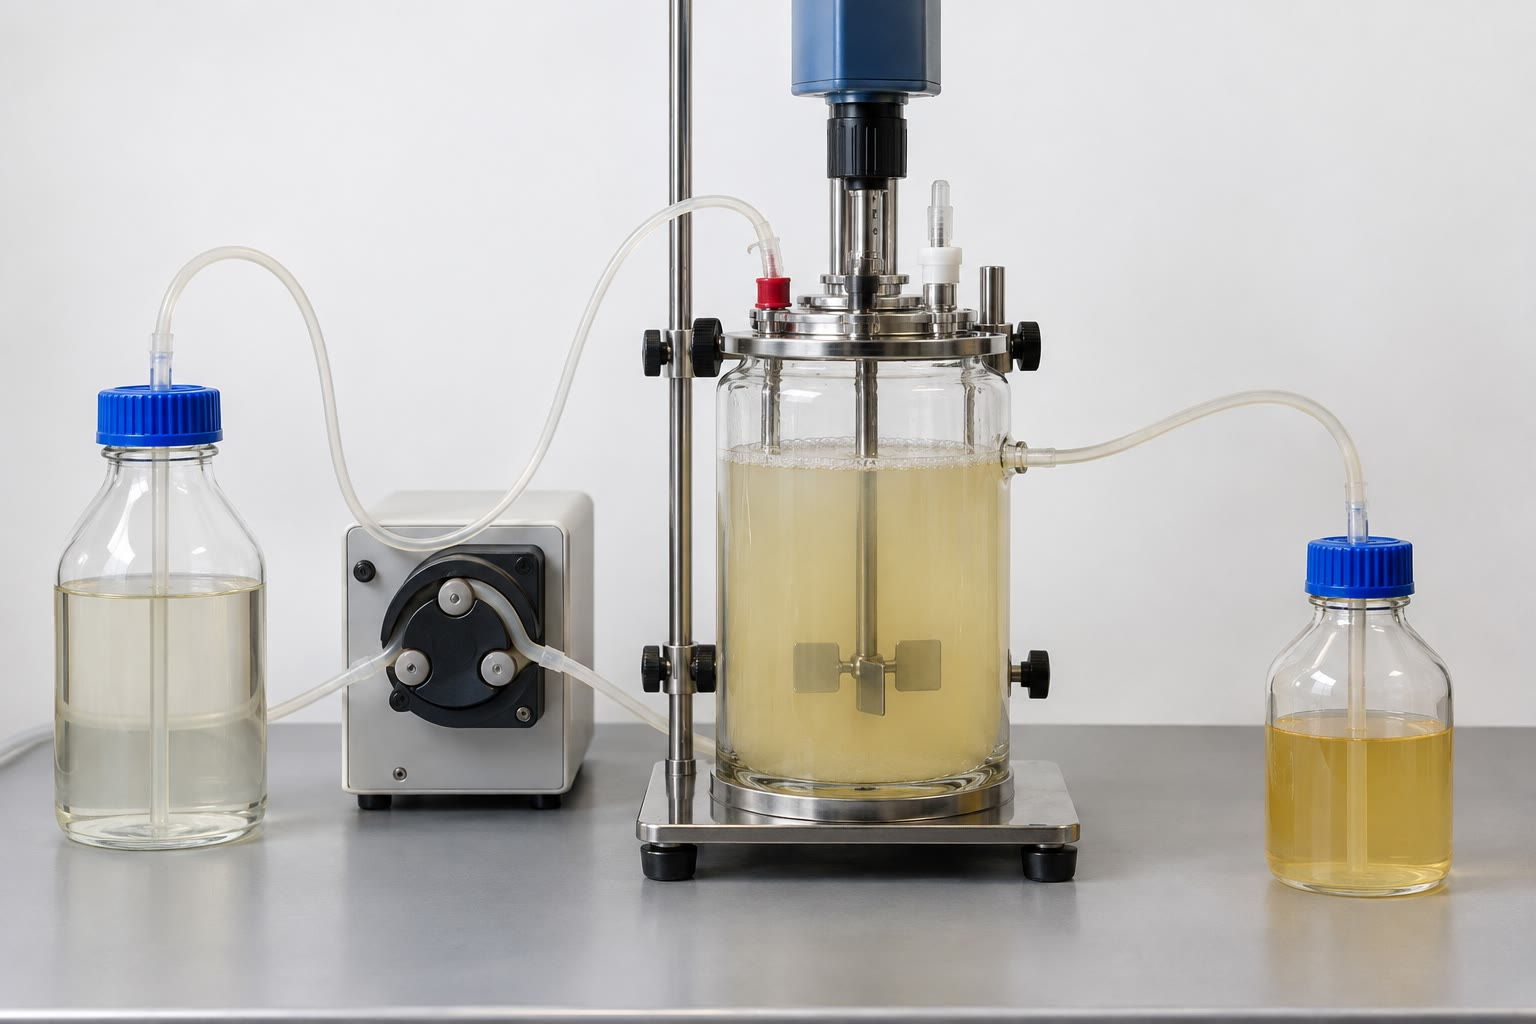
\includegraphics[width=0.6\linewidth]{images/book4/ai/b4-02-chemostat.jpg}

{\small Un chémostat de laboratoire~: le milieu neuf est pompé depuis le
réservoir de gauche, la culture déborde vers la droite~; la pompe fixe
le taux de croissance.}
\end{omfigure}

\begin{example}[Lire un chémostat]\label{ex:b2:microbial-metabolism:chemostat}
Avec $\mu_{\max} = \qty{1.0}{h^{-1}}$, $K_s = \qty{0.02}{g/L}$,
$S_{\text{in}} = \qty{2}{g/L}$ et $Y = 0.5$, pour $D =
\qty{0.5}{h^{-1}}$~: $S^* = 0.02\times 0.5/0.5 = \qty{0.02}{g/L}$ et
$X^* = 0.5\times 1.98 = \qty{0.99}{g/L}$~; la culture laisse
\qty{1}{\%} du sucre inutilisé. Le taux de lessivage vaut $1.0\times
2/2.02 = \qty{0.99}{h^{-1}}$. Un digesteur ou un intestin fonctionne sur
le même principe~: le côlon humain, alimenté trois fois par jour et vidé
une fois, maintient ses bactéries à un \omterm{thm:b2:microbial-metabolism:chemostat}{taux de dilution} voisin de
\qty{0.04}{h^{-1}}, et toute espèce incapable de doubler en un jour est
évacuée --- à moins qu'elle ne s'accroche à la paroi.
\end{example}

\section{Les biofilms}

\begin{definition}[Biofilm]\label{def:b2:microbial-metabolism:biofilm}
\index{biofilm}\index{matrice extracellulaire!bacterienne@bactérienne}
Un \emph{biofilm} est une communauté de micro-organismes fixés à une
surface et enrobés dans une \emph{matrice} qu'ils produisent eux-mêmes,
faite de polysaccharides, de protéines et d'ADN extracellulaire. Il se
forme par étapes~: \emph{adhésion} réversible de cellules isolées
(flagelles, pili), adhésion irréversible et croissance en
\emph{microcolonies}, \emph{maturation} en un film structuré avec des
tours et des canaux d'eau, et \emph{dispersion} de cellules qui s'en
vont à la nage ensemencer de nouvelles surfaces. La matrice retient
l'eau et les nutriments, protège les cellules de la dessiccation, des
brouteurs, des antibiotiques et des cellules immunitaires, et établit
des gradients chimiques qui font du film un paysage de niches. La
plupart des bactéries de la Terre vivent ainsi~: sur les rochers des
cours d'eau, sur les racines, sur les dents (la plaque dentaire), sur
les cathéters et les implants, dans les poumons des patients atteints
de mucoviscidose, sur les coques des navires et dans les canalisations.
\end{definition}

\begin{omfigure}
\begin{tikzpicture}[every node/.style={font=\scriptsize}]
  \fill[gray!35] (0,0) rectangle (13.6,0.35);
  \node at (6.8,0.17) {surface};
  % stage 1 attachment
  \foreach \p in {(0.6,0.55),(1.4,0.55)} \draw[thick, omDef, fill=omDef!30] \p ellipse (0.22 and 0.1);
  \draw[thick, omDef, fill=omDef!30] (1.0,1.6) ellipse (0.22 and 0.1);
  \draw[->, omDef] (1.0,1.45) -- (1.0,0.75);
  \node[below, align=center] at (1.1,-0.05) {1. adhésion};
  % stage 2 microcolony
  \begin{scope}[xshift=3.4cm]
    \fill[omExo!25] (0.15,0.35) .. controls (0.1,1.1) and (1.5,1.1) .. (1.45,0.35);
    \foreach \p in {(0.45,0.5),(0.8,0.5),(1.15,0.5),(0.6,0.75),(0.95,0.75),(0.8,0.95)} \draw[thick, omDef, fill=omDef!30] \p ellipse (0.18 and 0.09);
    \node[below, align=center] at (0.8,-0.05) {2. microcolonie,\\sécrétion de matrice};
  \end{scope}
  % stage 3 mature with channels
  \begin{scope}[xshift=6.8cm]
    \fill[omExo!25] (0.0,0.35) .. controls (0.2,1.9) and (0.9,2.2) .. (1.1,1.5) .. controls (1.2,0.9) and (1.4,0.6) .. (1.5,0.35);
    \fill[omExo!25] (1.7,0.35) .. controls (1.6,1.5) and (2.6,2.3) .. (2.9,1.2) .. controls (3.0,0.8) and (3.1,0.5) .. (3.2,0.35);
    \foreach \p in {(0.35,0.55),(0.7,0.55),(0.5,0.85),(0.8,1.15),(0.55,1.45),(2.0,0.6),(2.4,0.6),(2.2,0.9),(2.5,1.25),(2.3,1.6),(2.6,1.9),(2.1,1.3)} \draw[thick, omDef, fill=omDef!30] \p ellipse (0.16 and 0.08);
    \draw[<->, omThm, thick] (1.6,0.5) -- (1.6,1.6);
    \node[omThm, anchor=south] at (1.6,2.45) {canal d'eau};
    \node[below, align=center] at (1.6,-0.05) {3. film mature~: tours,\\canaux, gradients};
  \end{scope}
  % stage 4 dispersal
  \begin{scope}[xshift=11.2cm]
    \fill[omExo!25] (0.0,0.35) .. controls (0.1,1.5) and (1.0,1.6) .. (1.1,0.35);
    \foreach \p in {(0.3,0.55),(0.65,0.55),(0.5,0.85)} \draw[thick, omDef, fill=omDef!30] \p ellipse (0.16 and 0.08);
    \foreach \p/\a in {(1.4,1.5)/40,(1.9,1.1)/10,(1.6,2.0)/70} \draw[thick, omDef, fill=omDef!30, rotate around={\a:\p}] \p ellipse (0.16 and 0.08);
    \draw[->, omDef] (1.0,1.0) -- (1.35,1.35);
    \node[below, align=center] at (1.0,-0.05) {4. dispersion};
  \end{scope}
\end{tikzpicture}

{\small Le cycle de vie d'un \omterm{def:b2:microbial-metabolism:biofilm}{biofilm}~: des cellules isolées adhèrent,
forment des microcolonies qui sécrètent une matrice (en gris), mûrissent
en un film structuré avec des tours et des canaux d'eau, et libèrent des
cellules nageuses qui colonisent de nouvelles surfaces.}
\end{omfigure}

\begin{omfigure}
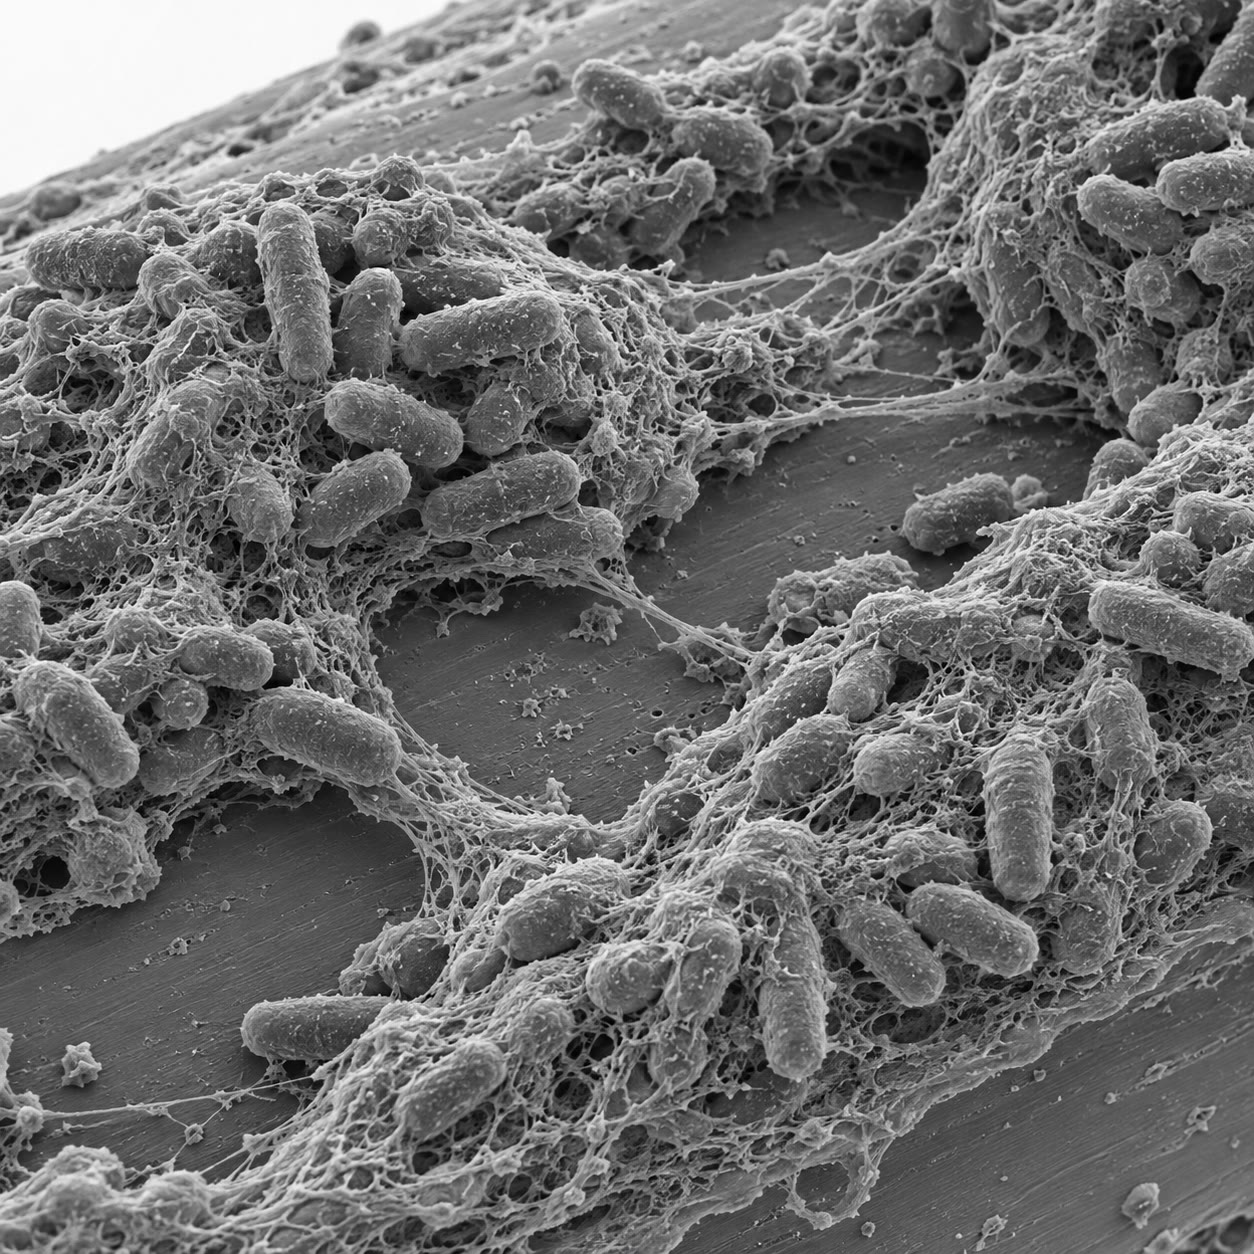
\includegraphics[width=0.46\linewidth]{images/book4/ai/b4-02-biofilm-sem.jpg}

{\small Un \omterm{def:b2:microbial-metabolism:biofilm}{biofilm} sur un cathéter, observé en microscopie électronique à
balayage~: des bactéries en bâtonnet enrobées dans la matrice fibreuse
qu'elles ont sécrétée, avec des canaux ouverts entre les amas.}
\end{omfigure}

\begin{theorem}[Les gradients dans un biofilm]\label{thm:b2:microbial-metabolism:gradient}
\index{profondeur de penetration du dioxygene@profondeur de pénétration du dioxygène}
Dans un film d'épaisseur $L$ dont les cellules consomment le dioxygène
à un taux volumique constant $q$, la concentration étant maintenue à
$c_0$ à la surface et aucun flux ne traversant le support, le profil
stationnaire du dioxygène est une parabole et, si le film est assez
épais pour que le dioxygène s'épuise, il s'épuise à la
\emph{profondeur de pénétration}
\[
L_p = \sqrt{\frac{2 D_e\, c_0}{q}},
\]
où $D_e$ est le coefficient de diffusion effectif dans la matrice.
Avec $D_e = \qty{1.5e-9}{m^2/s}$, $c_0 = \qty{0.25}{mol/m^3}$ et $q
= \qty{0.17}{mol/m^3/s}$ (un film dense de cellules qui respirent), $L_p
\approx \qty{66}{\micro m}$~: au-delà d'un dixième de millimètre de
profondeur, un \omterm{def:b2:microbial-metabolism:biofilm}{biofilm} est anoxique, et dénitrifiants, fermenteurs et
sulfato-réducteurs vivent sous un toit d'aérobies.
\end{theorem}
\begin{proof}
Soit $x$ la profondeur sous la surface. En régime stationnaire, le flux
diffusif $-D_e\,\mathrm{d}c/\mathrm{d}x$ ne varie avec la profondeur
que du fait de la consommation~: $D_e\,\mathrm{d}^2c/\mathrm{d}x^2 = q$.
En intégrant deux fois, $c = c_0 + a x + q x^2/2D_e$. Si le dioxygène
s'annule à la profondeur $L_p$ avec un flux nul en ce point (rien
n'arrive d'en dessous),
$c(L_p) = 0$ et $c'(L_p) = 0$~: la seconde condition donne
$a = -qL_p/D_e$, et la première donne alors
$c_0 - qL_p^2/D_e + qL_p^2/2D_e = 0$, c'est-à-dire
$L_p^2 = 2D_e c_0/q$. Le profil est $c = (q/2D_e)(L_p - x)^2$.
\end{proof}

\begin{omfigure}
\begin{tikzpicture}
\begin{axis}[
  width=0.78\linewidth, height=5.6cm,
  axis x line=bottom, axis y line=left,
  xmin=0, xmax=120, ymin=0, ymax=0.28,
  xlabel={profondeur dans le film (\unit{\micro m})}, ylabel={$\mathrm{O_2}$ (\unit{mol/m^3})},
  xlabel style={font=\small, at={(axis description cs:0.5,-0.14)}, anchor=north},
  ylabel style={font=\small},
  tick label style={font=\small}, xtick={0,20,40,60,80,100,120}, ytick={0,0.1,0.2},
  clip=false,
]
\addplot[very thick, omDef, domain=0:66, samples=60] {0.25*(1-x/66)^2};
\addplot[very thick, omDef, domain=66:120, samples=2] {0};
\fill[omThm!12] (axis cs:66,0) rectangle (axis cs:120,0.28);
\node[font=\scriptsize, anchor=north, align=center] at (axis cs:93,0.27) {zone anoxique~:\\dénitrifiants, fermenteurs,\\sulfato-réducteurs};
\draw[dashed, gray] (axis cs:66,0) -- (axis cs:66,0.28); \node[font=\scriptsize, anchor=south] at (axis cs:66,0.28) {$L_p$};
\node[font=\scriptsize, anchor=west] at (axis cs:24,0.18) {zone aérobie};
\end{axis}
\end{tikzpicture}

{\small Le dioxygène dans un \omterm{def:b2:microbial-metabolism:biofilm}{biofilm} qui respire~: une décroissance
parabolique depuis la valeur du milieu à la surface jusqu'à zéro à la
profondeur de pénétration, \qty{66}{\micro m} pour les valeurs du
théorème. Tout ce qui est plus profond est anoxique.}
\end{omfigure}

\begin{proposition}[La détection du quorum]\label{prop:b2:microbial-metabolism:quorum}
\index{detection du quorum@détection du quorum}\index{auto-inducteur}
Les bactéries se comptent. Chaque cellule sécrète à faible débit
constant une petite molécule signal, un \emph{auto-inducteur}
(acyl-homosérine lactones chez les bactéries à Gram négatif, courts
peptides chez les bactéries à Gram positif). Dans une suspension
diluée, le signal diffuse au loin~; dans une population dense ou un
\omterm{def:b2:microbial-metabolism:biofilm}{biofilm}, il s'accumule et, au-delà d'une concentration seuil, se fixe à
un récepteur qui active un ensemble de gènes
--- dont le gène de l'auto-inducteur lui-même, d'où son nom.
Les gènes ainsi contrôlés sont ceux qui ne sont rentables que si de
nombreuses cellules agissent ensemble~: la luminescence, la sécrétion
d'enzymes digestives et de toxines, la production de matrice, la
virulence des pathogènes qui doivent submerger un hôte d'un seul coup
plutôt que de l'alerter une cellule à la fois.
\end{proposition}
\begin{proof}[Faits expérimentaux]
Nealson, Platt et Hastings (1970) montrèrent que la bactérie marine
\emph{Vibrio fischeri}, qui éclaire l'organe lumineux d'un calmar, reste
obscure en culture diluée et ne luit qu'au-delà d'environ $10^{7}$
cellules par millilitre~; du milieu débarrassé des cellules, prélevé
dans une culture dense et lumineuse, faisait aussitôt luire une culture
diluée. Le milieu contenait le signal~; sa structure, une acyl-homosérine
lactone, fut déterminée en 1981, et les mutants incapables de la
fabriquer ne luisent jamais, quelle que soit leur densité.
\end{proof}

\begin{example}[Pourquoi un biofilm survit aux antibiotiques]\label{ex:b2:microbial-metabolism:tolerance}
Les cellules d'un \omterm{def:b2:microbial-metabolism:biofilm}{biofilm} survivent à des concentrations d'antibiotique
cent à mille fois supérieures à celles qui tuent la même souche en
suspension, sans aucun gène de résistance. La matrice ralentit la
diffusion du médicament et en fixe une partie~; les gradients laissent
les cellules profondes affamées, anoxiques et presque sans croissance,
or la plupart des antibiotiques ne tuent que les cellules en croissance
(les pénicillines exigent la synthèse de la paroi, les aminosides un
transport actif)~; quelques cellules \emph{persistantes} sont
entièrement dormantes et reconstituent le film à l'arrêt du traitement.
Une infection chronique sur un implant se traite donc en général par le
retrait de l'implant.
\end{example}

\section{Les communautés microbiennes}

\begin{example}[La colonne de Winogradsky, expliquée]\label{ex:b2:microbial-metabolism:column}
La lumière et l'air entrent par le haut~; la matière organique et le
sulfate viennent de la vase. Cyanobactéries et algues croissent au
sommet et libèrent du dioxygène. En dessous, les hétérotrophes épuisent
le dioxygène sur la matière organique, puis le nitrate~; plus bas, les
sulfato-réducteurs transforment le sulfate en sulfure, qui diffuse vers
le haut et noircit la vase de sulfure de fer. Là où le sulfure qui monte
rencontre la lumière qui descend, les bactéries pourpres sulfureuses
l'oxydent par photosynthèse (la bande pourpre), les bactéries vertes
sulfureuses en dessous d'elles~; là où le sulfure rencontre le
dioxygène, à l'obscurité, des sulfo-oxydants incolores comme
\emph{Beggiatoa} vivent de \omterm{def:b2:microbial-metabolism:trophic}{chimiolithotrophie} (le voile blanc)~; là où
le fer réduit rencontre le dioxygène, les ferro-oxydants laissent une
bande couleur rouille. Le soufre circule entre sulfure et sulfate dans
la colonne~; le carbone circule entre
$\mathrm{CO_2}$ et matière organique~; seule la lumière entre et seule
la chaleur sort. C'est un écosystème fermé au bilan énergétique ouvert,
et un modèle réduit du fond de l'océan.
\end{example}

\begin{omfigure}
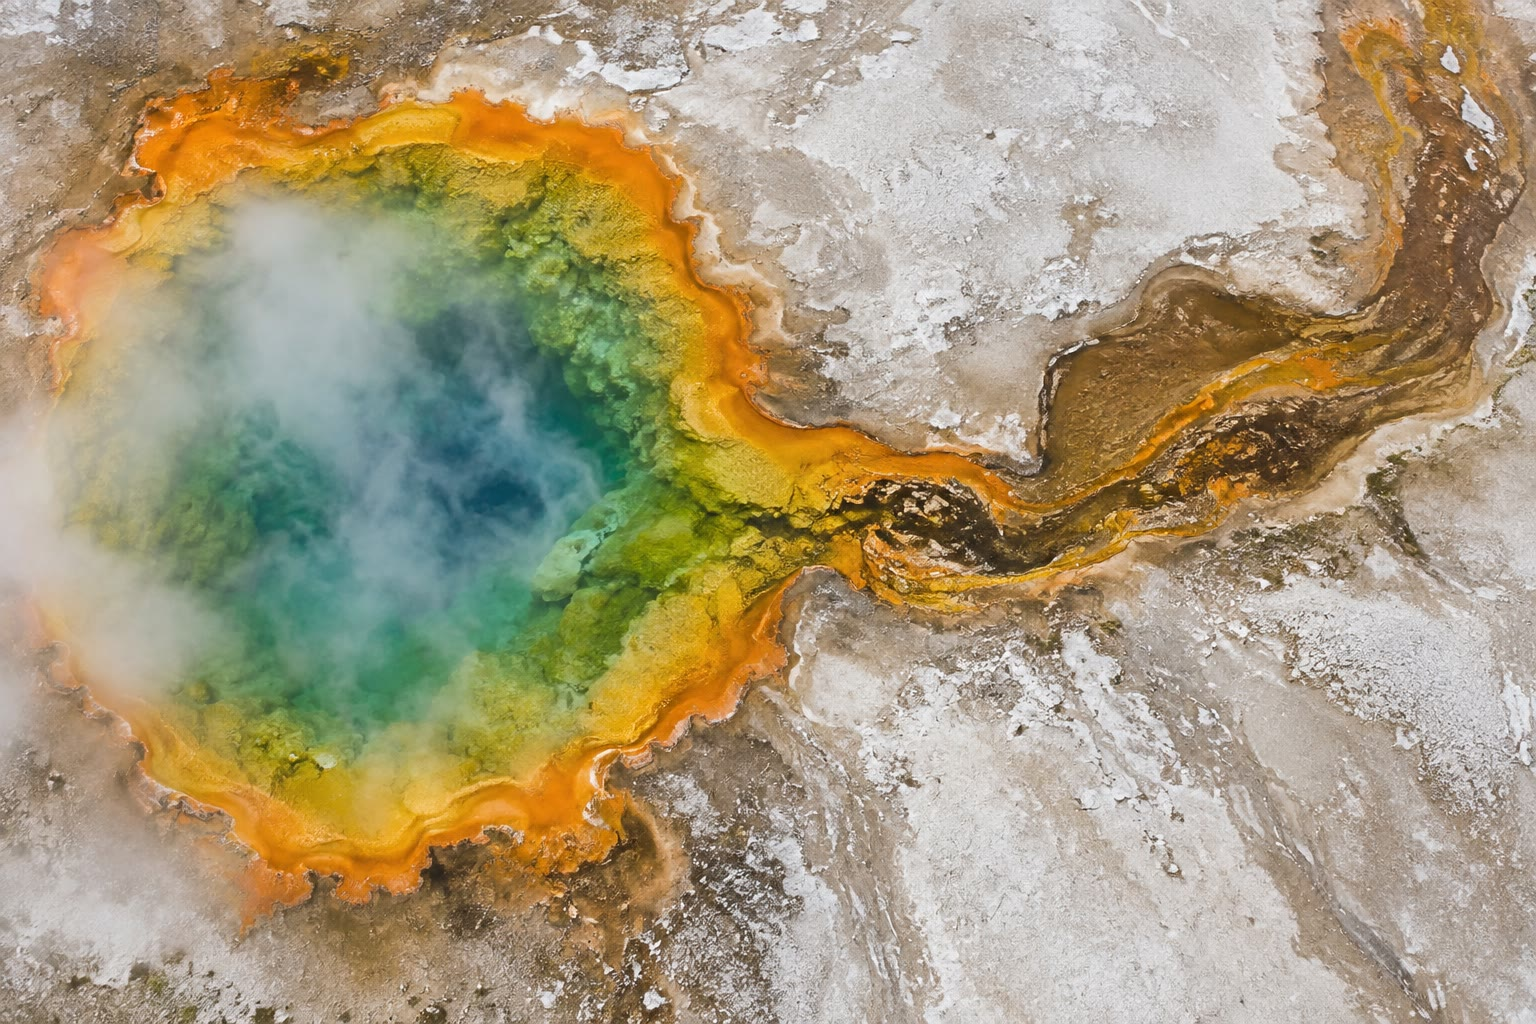
\includegraphics[width=0.62\linewidth]{images/book4/ai/b4-02-hot-spring-mats.jpg}

{\small Des tapis microbiens autour d'une source chaude~: chaque couleur
est une population qui vit à la température et dans la chimie de sa
bande --- cyanobactéries thermophiles et bactéries vertes dans
l'écoulement plus frais, \omterm{def:b2:microbial-metabolism:trophic}{chimiolithotrophes} incolores dans l'eau la plus
chaude.}
\end{omfigure}

\begin{remark}[Les tapis microbiens et la Terre primitive]\label{rem:b2:microbial-metabolism:mats}
Autour des sources chaudes et sur les estrans, des tapis microbiens
stratifiés de quelques millimètres d'épaisseur ramassent toute la
colonne dans une épaisseur que la lumière peut traverser~:
cyanobactéries au-dessus, bactéries pourpres en dessous,
sulfato-réducteurs à la base, chaque couche consommant ce que produit
celle du dessus, et le tapis remontant à travers le sédiment qu'il
piège. Les tapis fossiles --- les stromatolithes --- sont les plus
anciennes traces de vie, vieilles de \num{3.5} milliards d'années.
Pendant deux milliards d'années, avant les plantes et les animaux, la
biosphère fut constituée de ces tapis et du plancton qui les
surmontait, et ce sont eux qui remplirent l'air de dioxygène
(\cref{ch:b2:biogeochemical-cycles}).
\end{remark}

\section{Exercices}

\begin{exercise}[$\star$]\label{exo:b2:microbial-metabolism:1}
Classer selon la source d'énergie, la source d'électrons et la source
de carbone~: une cyanobactérie~; \emph{Nitrosomonas}~; \emph{E.~coli}
sur glucose~; une bactérie pourpre non sulfureuse cultivée à la lumière
sur succinate~; \emph{Thiobacillus} sur $\mathrm{H_2S}$ à l'obscurité.
\end{exercise}

\begin{exercise}[$\star$]\label{exo:b2:microbial-metabolism:2}
Énumérer les accepteurs d'électrons de la respiration par ordre de
rendement énergétique décroissant, et dire où chacun est utilisé dans
un sédiment.
\end{exercise}

\begin{exercise}[$\star$]\label{exo:b2:microbial-metabolism:3}
Équilibrer l'oxydation du glucose en $\mathrm{CO_2}$ par le nitrate
réduit en $\mathrm{N_2}$ (en solution acide, l'eau étant l'autre
produit). Combien d'ions nitrate faut-il par glucose~?
\end{exercise}

\begin{exercise}[$\star$]\label{exo:b2:microbial-metabolism:4}
Définir un \omterm{def:b2:microbial-metabolism:biofilm}{biofilm} et nommer ses quatre étapes. Donner trois situations
où les \omterm{def:b2:microbial-metabolism:biofilm}{biofilms} comptent pour la santé humaine ou pour l'industrie.
\end{exercise}

\begin{exercise}[$\star\star$]\label{exo:b2:microbial-metabolism:5}
Calculer $\Delta G^{\circ\prime}$ pour $4\mathrm{H_2} + \mathrm{CO_2}
\to \mathrm{CH_4} + 2\mathrm{H_2O}$ à partir des potentiels
$\mathrm{2H^+/H_2}$ (\qty{-0.42}{V}) et $\mathrm{CO_2/CH_4}$
(\qty{-0.24}{V}). Combien d'ATP (à \qty{50}{kJ/mol}) un méthanogène
peut-il au plus produire par $\mathrm{H_2}$~? Commenter sa vitesse de
croissance.
\end{exercise}

\begin{exercise}[$\star\star$]\label{exo:b2:microbial-metabolism:6}
Une bactérie a $\mu_{\max} = \qty{1.2}{h^{-1}}$ et $K_s =
\qty{5}{mg/L}$ de glucose. Calculer $\mu$ et le \omterm{def:b2:unicellular-diversity:division}{temps de génération} à
1, 5 et \qty{50}{mg/L}. À quelle concentration croît-elle à
\qty{90}{\%} de son maximum~?
\end{exercise}

\begin{exercise}[$\star\star$]\label{exo:b2:microbial-metabolism:7}
Un chémostat avec $\mu_{\max} = \qty{0.8}{h^{-1}}$, $K_s =
\qty{0.05}{g/L}$, $S_{\text{in}} = \qty{5}{g/L}$, $Y = 0.4$ fonctionne à
$D = \qty{0.4}{h^{-1}}$. Calculer $S^*$, $X^*$, la production de
biomasse par litre et par heure, et le taux de lessivage.
\end{exercise}

\begin{exercise}[$\star\star$]\label{exo:b2:microbial-metabolism:8}
L'oxydation d'un $\mathrm{NH_4^+}$ en nitrite fournit \qty{275}{kJ}~; un
nitrifiant en capte le quart sous forme d'ATP (\qty{50}{kJ/mol}), et la
fixation d'un $\mathrm{CO_2}$ en biomasse coûte l'équivalent de 12
ATP. Combien d'ions ammonium doit-il oxyder par carbone fixé~? Pourquoi
le rendement d'un nitrifiant est-il si faible comparé à celui d'un
hétérotrophe~?
\end{exercise}

\begin{exercise}[$\star\star$]\label{exo:b2:microbial-metabolism:9}
Calculer la \omterm{thm:b2:microbial-metabolism:gradient}{profondeur de pénétration du dioxygène} dans un \omterm{def:b2:microbial-metabolism:biofilm}{biofilm} avec
$D_e =
\qty{1.2e-9}{m^2/s}$, $c_0 = \qty{0.20}{mol/m^3}$ et $q =
\qty{0.5}{mol/m^3/s}$. Que devient $L_p$ si le dioxygène du milieu est
doublé~? Si les cellules respirent quatre fois plus vite~?
\end{exercise}

\begin{exercise}[$\star\star\star$]\label{exo:b2:microbial-metabolism:10}
Prévoir les bandes d'une colonne de Winogradsky de haut en bas, en
nommant le métabolisme de chacune, et expliquer (a) pourquoi la bande
pourpre se forme là où elle se forme, (b) pourquoi la vase noircit,
(c) en quel sens la colonne est un système fermé et en quel sens un
système ouvert.
\end{exercise}

\begin{exercise}[$\star\star\star$]\label{exo:b2:microbial-metabolism:11}
Chaque cellule d'une population de densité $n$ (cellules par litre)
sécrète un auto-inducteur à raison de $p = 5$ molécules par seconde~; la
molécule est dégradée avec une constante de vitesse $k = \qty{5e-4}{s^{-1}}$.
Écrire la concentration stationnaire $A^*$ en fonction de $n$. Le
récepteur s'active à $A_c = \qty{10}{nmol/L}$~: calculer la densité seuil
en cellules par millilitre. La comparer à celle d'une culture dense
($10^{9}$ par millilitre) et de l'eau de mer ($10^{5}$ par millilitre),
et expliquer pourquoi un \omterm{def:b2:microbial-metabolism:biofilm}{biofilm} atteint le quorum dans un volume où une
suspension ne l'atteindrait jamais.
\end{exercise}

\begin{exercise}[$\star\star\star$]\label{exo:b2:microbial-metabolism:12}
«~Les \omterm{def:b2:unicellular-diversity:prokaryote}{procaryotes} font tourner la chimie de la planète.~» Discuter cette
affirmation à l'aide de trois processus de ce chapitre qu'aucun
eucaryote ne peut réaliser, en disant pour chacun ce qui arriverait à
la biosphère s'il cessait.
\end{exercise}

\section{Problème~: une station d'épuration}

\begin{problem}[{Problème du week-end --- la station d'épuration d'une ville
analysée comme un ensemble de réacteurs microbiens, de l'énergétique de
ses bactéries au méthane qui l'alimente, jusqu'au bilan énergétique de
la station}]
\label{pb:b2:microbial-metabolism:1}
Une station traite $Q = \qty{10000}{m^3}$ d'eaux usées par jour,
chargées de \qty{300}{g/m^3} de matière organique, mesurée par le
dioxygène nécessaire pour la brûler (sa \emph{demande chimique en
oxygène}, DCO), et de \qty{40}{g/m^3} d'azote ammoniacal. Elle comprend
un bassin aéré de boues activées, un bassin anoxique de \omterm{def:b2:microbial-metabolism:anaerobic}{dénitrification}
et un digesteur anaérobie pour les boues. Données~: les hétérotrophes
aérobies convertissent la matière organique avec un rendement $Y = 0.4$
(kilogramme de DCO de biomasse par kilogramme de DCO de substrat, le
reste étant oxydé)~; la nitrification exige \qty{4.57}{kg} de
$\mathrm{O_2}$ par kilogramme d'azote~; la \omterm{def:b2:microbial-metabolism:anaerobic}{dénitrification} exige
\qty{2.86}{kg} de DCO de substrat par kilogramme d'azote nitrique~;
l'aération fournit \qty{2}{kg} de
$\mathrm{O_2}$ par kilowattheure~; la DCO des boues est convertie en
méthane dans le digesteur à \qty{60}{\%}, chaque kilogramme de DCO
converti donnant \qty{0.35}{m^3} de méthane de contenu énergétique
\qty{36}{MJ/m^3}, brûlé dans un groupe électrogène de rendement
électrique \qty{35}{\%}. Nitrifiants~: $\mu_{\max} = \qty{0.5}{d^{-1}}$, $K_s =
\qty{1}{g/m^3}$ d'azote ammoniacal.

\medskip
\noindent\textbf{Partie I --- L'énergétique.}
\begin{enumerate}
  \item À l'aide de la \omterm{thm:b2:microbial-metabolism:redox}{tour à électrons}, calculer $\Delta G^{\circ\prime}$
        pour l'oxydation d'une mole de glucose (24 électrons à
        \qty{-0.43}{V}) par le dioxygène (\qty{+0.82}{V}).
  \item Le calculer pour le nitrate réduit en $\mathrm{N_2}$
        (\qty{+0.74}{V}) et pour le sulfate réduit en sulfure
        (\qty{-0.22}{V}).
  \item Pourquoi la \omterm{def:b2:microbial-metabolism:anaerobic}{dénitrification} ne démarre-t-elle que dans le bassin
        anoxique, et pourquoi la \omterm{def:b2:microbial-metabolism:anaerobic}{sulfato-réduction} (avec son odeur)
        est-elle le signe d'une station mal conduite~?
  \item Si les cellules captent \qty{40}{\%} de l'énergie libre sous
        forme d'ATP (\qty{50}{kJ/mol}), combien d'ATP par glucose
        chacun des trois métabolismes fournit-il~?
  \item Combien de fois plus de glucose un sulfato-réducteur doit-il
        traiter qu'un aérobie pour une même croissance~?
  \item Les fermenteurs du digesteur obtiennent 2 ATP par glucose.
        Expliquer pourquoi le digesteur produit néanmoins presque pas de
        biomasse, et surtout du gaz.
\end{enumerate}

\medskip
\noindent\textbf{Partie II --- Le bassin aéré.}
\begin{enumerate}[resume]
  \item Calculer la charge journalière en matière organique, en
        kilogrammes de DCO.
  \item Calculer la biomasse produite par jour (en DCO) et le dioxygène
        nécessaire pour oxyder le reste.
  \item Calculer l'énergie d'aération pour la matière organique, en
        kilowattheures par jour.
  \item Calculer la charge journalière en azote et le dioxygène
        nécessaire pour le nitrifier.
  \item Les boues sont retenues dans le bassin pendant un temps moyen
        $\theta$ (l'inverse de leur \omterm{thm:b2:microbial-metabolism:chemostat}{taux de dilution}). En dessous de quel
        $\theta$ les nitrifiants sont-ils lessivés, quelle que soit la
        concentration en ammonium~?
  \item Avec $\theta = \qty{10}{d}$, calculer la concentration résiduelle
        en ammonium dans l'effluent.
  \item L'hiver abaisse $\mu_{\max}$ à \qty{0.25}{d^{-1}}. Recalculer
        l'ammonium résiduel et dire ce que doit faire l'exploitant.
\end{enumerate}

\medskip
\noindent\textbf{Partie III --- La \omterm{def:b2:microbial-metabolism:anaerobic}{dénitrification} et le digesteur.}
Le nitrate produit dans le bassin aéré est recyclé vers le bassin
anoxique, où des hétérotrophes le réduisent avec la matière organique
entrante.
\begin{enumerate}[resume]
  \item Calculer la matière organique (kilogrammes de DCO par jour)
        consommée par la \omterm{def:b2:microbial-metabolism:anaerobic}{dénitrification} de tout l'azote.
  \item Calculer la masse d'azote libérée dans l'air sous forme de
        $\mathrm{N_2}$ par jour, et la masse qui quitte la station dans
        l'effluent sous forme d'ammonium (question 12), en fraction de la
        charge.
  \item Cette matière organique n'a plus besoin d'aération. Calculer le
        dioxygène économisé, et la demande totale en dioxygène de la
        station (matière organique restante plus nitrification).
  \item Les boues produites (question 8, comptées en DCO) partent au
        digesteur. Calculer le méthane produit par jour.
  \item Calculer l'énergie de ce méthane et l'électricité qu'il fournit.
  \item Calculer l'électricité d'aération correspondant à la demande
        totale en dioxygène de la question 16, et comparer.
\end{enumerate}

\medskip
\noindent\textbf{Partie IV --- Le réacteur à \omterm{def:b2:microbial-metabolism:biofilm}{biofilm}.}
Un lit bactérien fait croître un \omterm{def:b2:microbial-metabolism:biofilm}{biofilm} sur des pierres~; l'eau
contient \qty{0.2}{mol/m^3} de dioxygène, $D_e = \qty{1.5e-9}{m^2/s}$, et
le film respire à $q = \qty{0.3}{mol/m^3/s}$.
\begin{enumerate}[resume]
  \item Établir le profil de dioxygène $c(x)$ dans un film assez épais
        pour devenir anoxique.
  \item Calculer la profondeur de pénétration.
  \item Le film a \qty{300}{\micro m} d'épaisseur. Quelle fraction en est
        aérobie, et que font les cellules situées en dessous du nitrate
        qui diffuse depuis la couche aérobie~?
  \item Expliquer pourquoi un même \omterm{def:b2:microbial-metabolism:biofilm}{biofilm} peut nitrifier et dénitrifier
        à la fois, ce que le bassin aéré ne peut pas faire.
  \item On ajoute du chlore pour désinfecter l'effluent. Donner deux
        raisons pour lesquelles le \omterm{def:b2:microbial-metabolism:biofilm}{biofilm} survit à une dose qui tue les
        mêmes bactéries en suspension.
  \item Énoncer le résultat~: la demande journalière de la station en
        dioxygène, sa production de méthane, et la fraction de son
        électricité d'aération que fournit le méthane.
\end{enumerate}
\end{problem}
